\chapter{Background}

\section{Non-natural images}

\subsection{Vector graphics}
In contrast to raster images, which encode color values for each point (or \textit{pixel}) in an image, vector graphics describe a parameterized set of curves and shapes.

Many specifications exist for describing images in vector format, including Scalable Vector Graphics (SVG), Encapsulated PostScript (EPS), and Adobe PDF.

\begin{figure}[t]
    \subcaptionbox{Raster images are defined as two-dimensional arrays of pixel values, while vector graphics define curves and paths mathematically. Thus, when scaled, vector graphics (right) can still be rendered smoothly while raster images (left) degrade in quality.\label{fig:svg-a}}{
\includegraphics[height=2in]{figures/b_vs_vec}} \quad
    \subcaptionbox{SVG is an XML-based markup language that describes geometric elements within a vector image. A single path is used to draw this soap bubble, and colored curves in the image correspond approximately to the highlighted attribute commands that describe them. For example, the command \code{l-0.69-1.32} indicates a line drawn from a starting point to a point 0.69 units to the left and 1.32 units down.\label{fig:svg-b}}{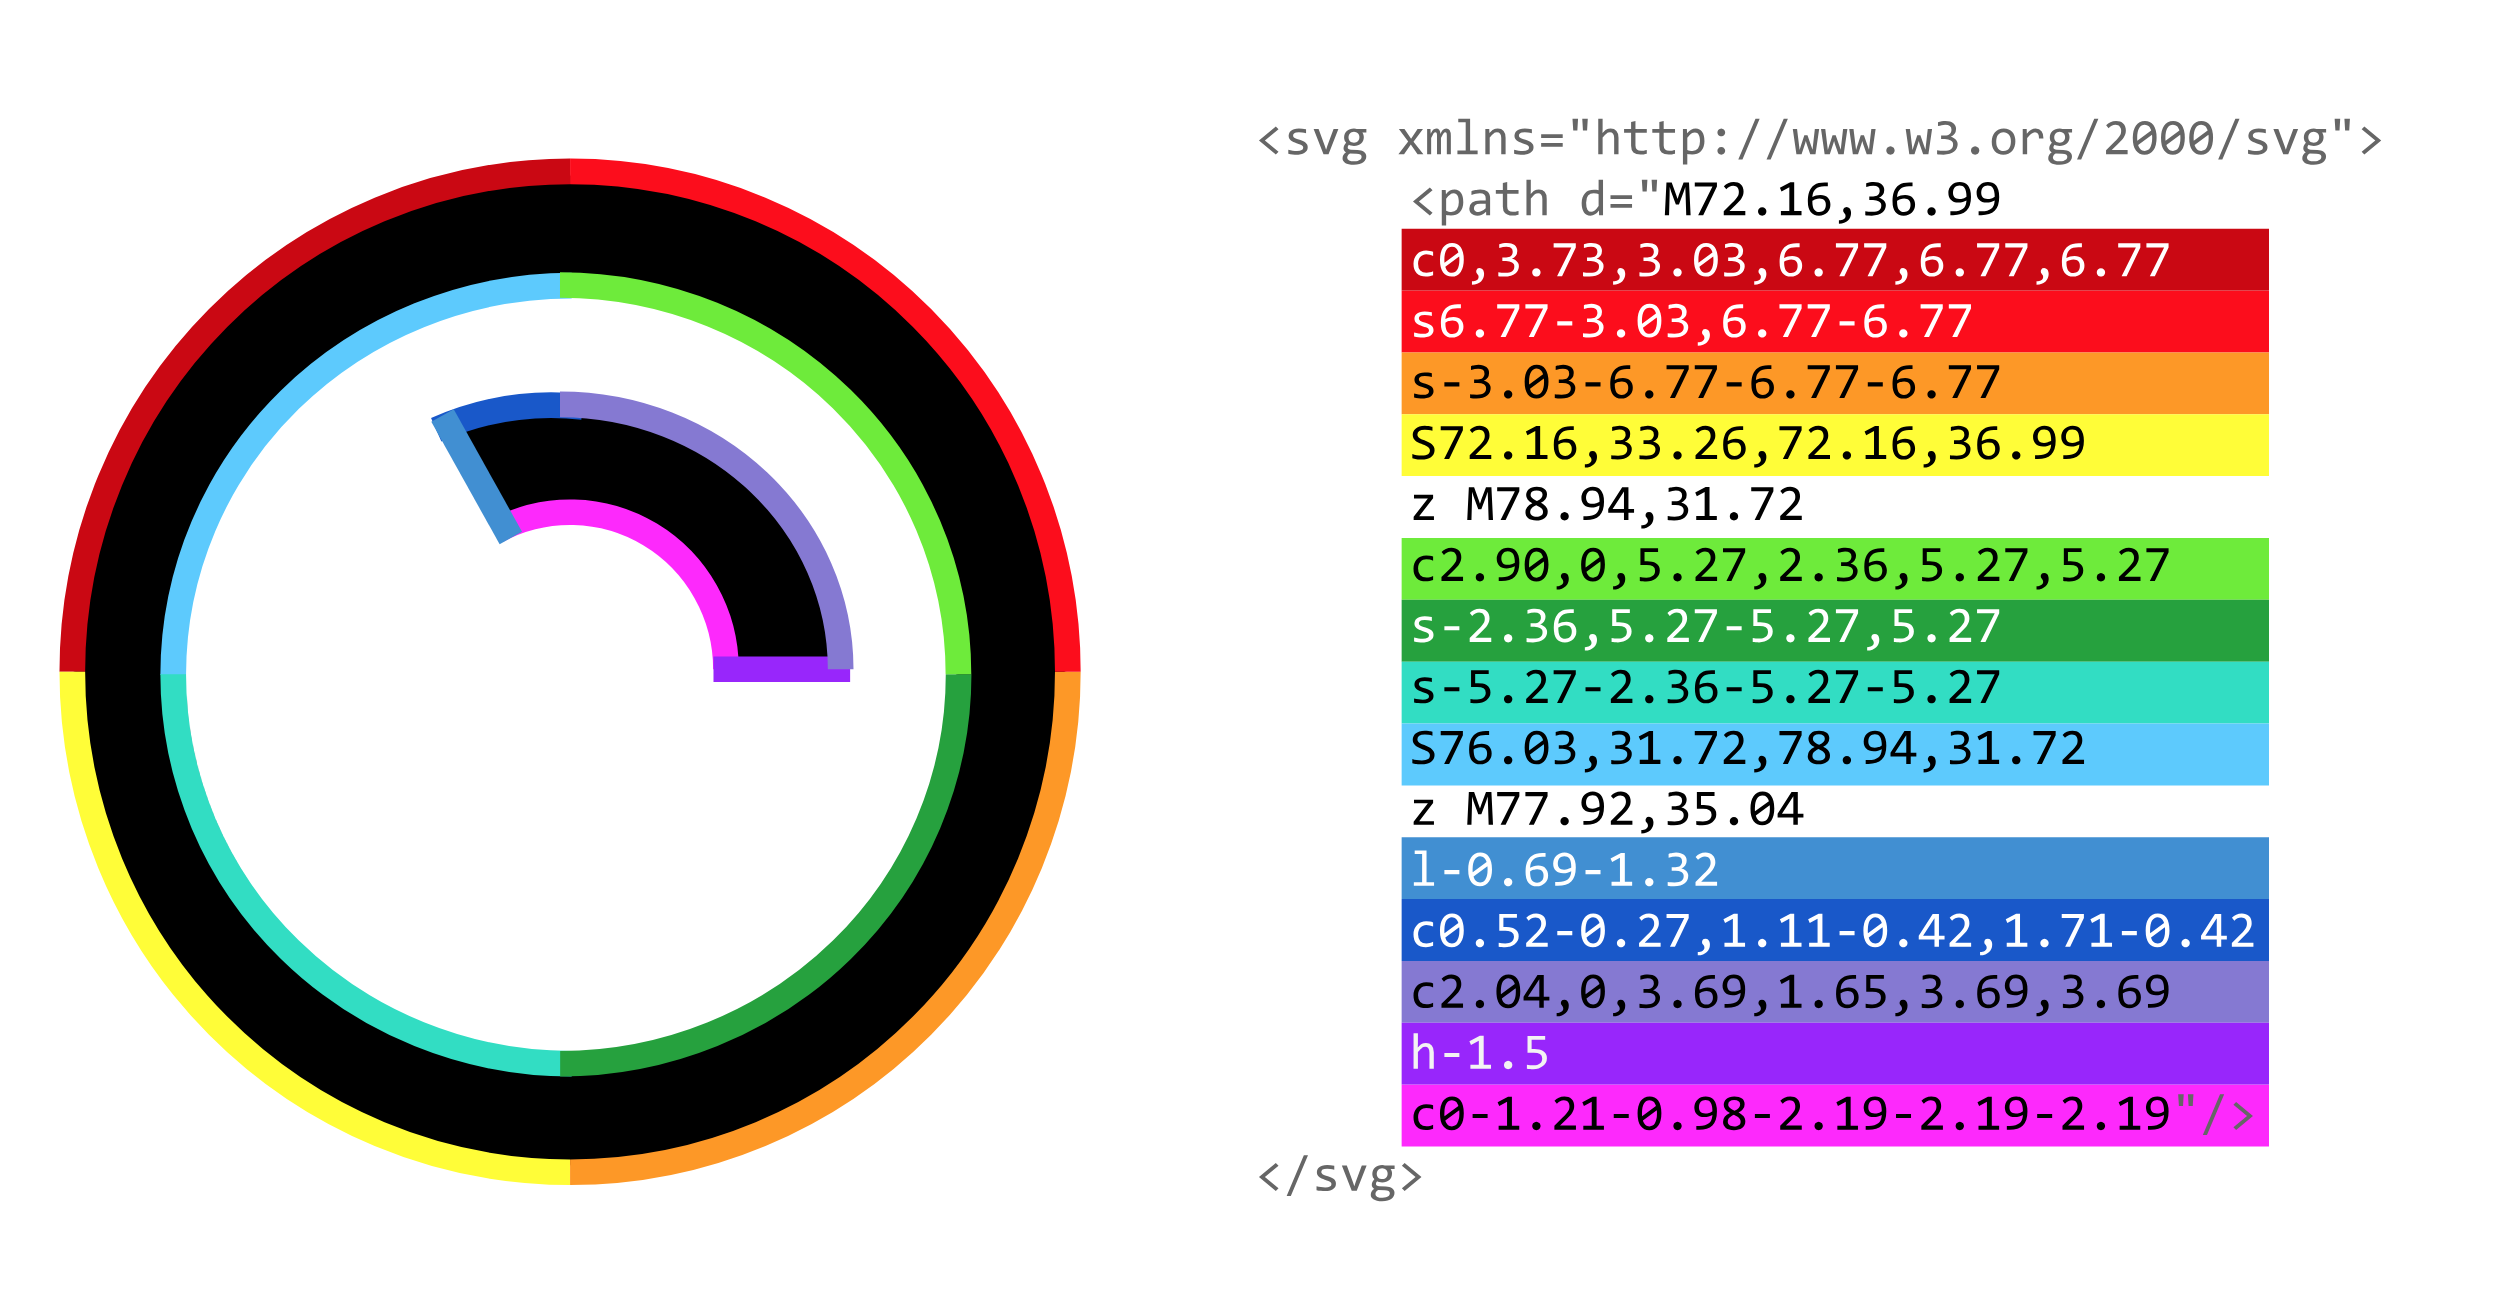
\includegraphics[height=2in]{figures/svgs}}
    \caption[An overview of the specification for scalable vector graphics (SVG)]{a visual comparison of raster and vector graphics. Figure~\ref{fig:svg-b} walks through a sample vector graphics path. Image source: \textit{Dog Wash} by Llisole from the Noun Project.\label{fig:svg}}
\end{figure}

\subsection{Icons}
\subsection{Font faces}

\begin{figure}[]
	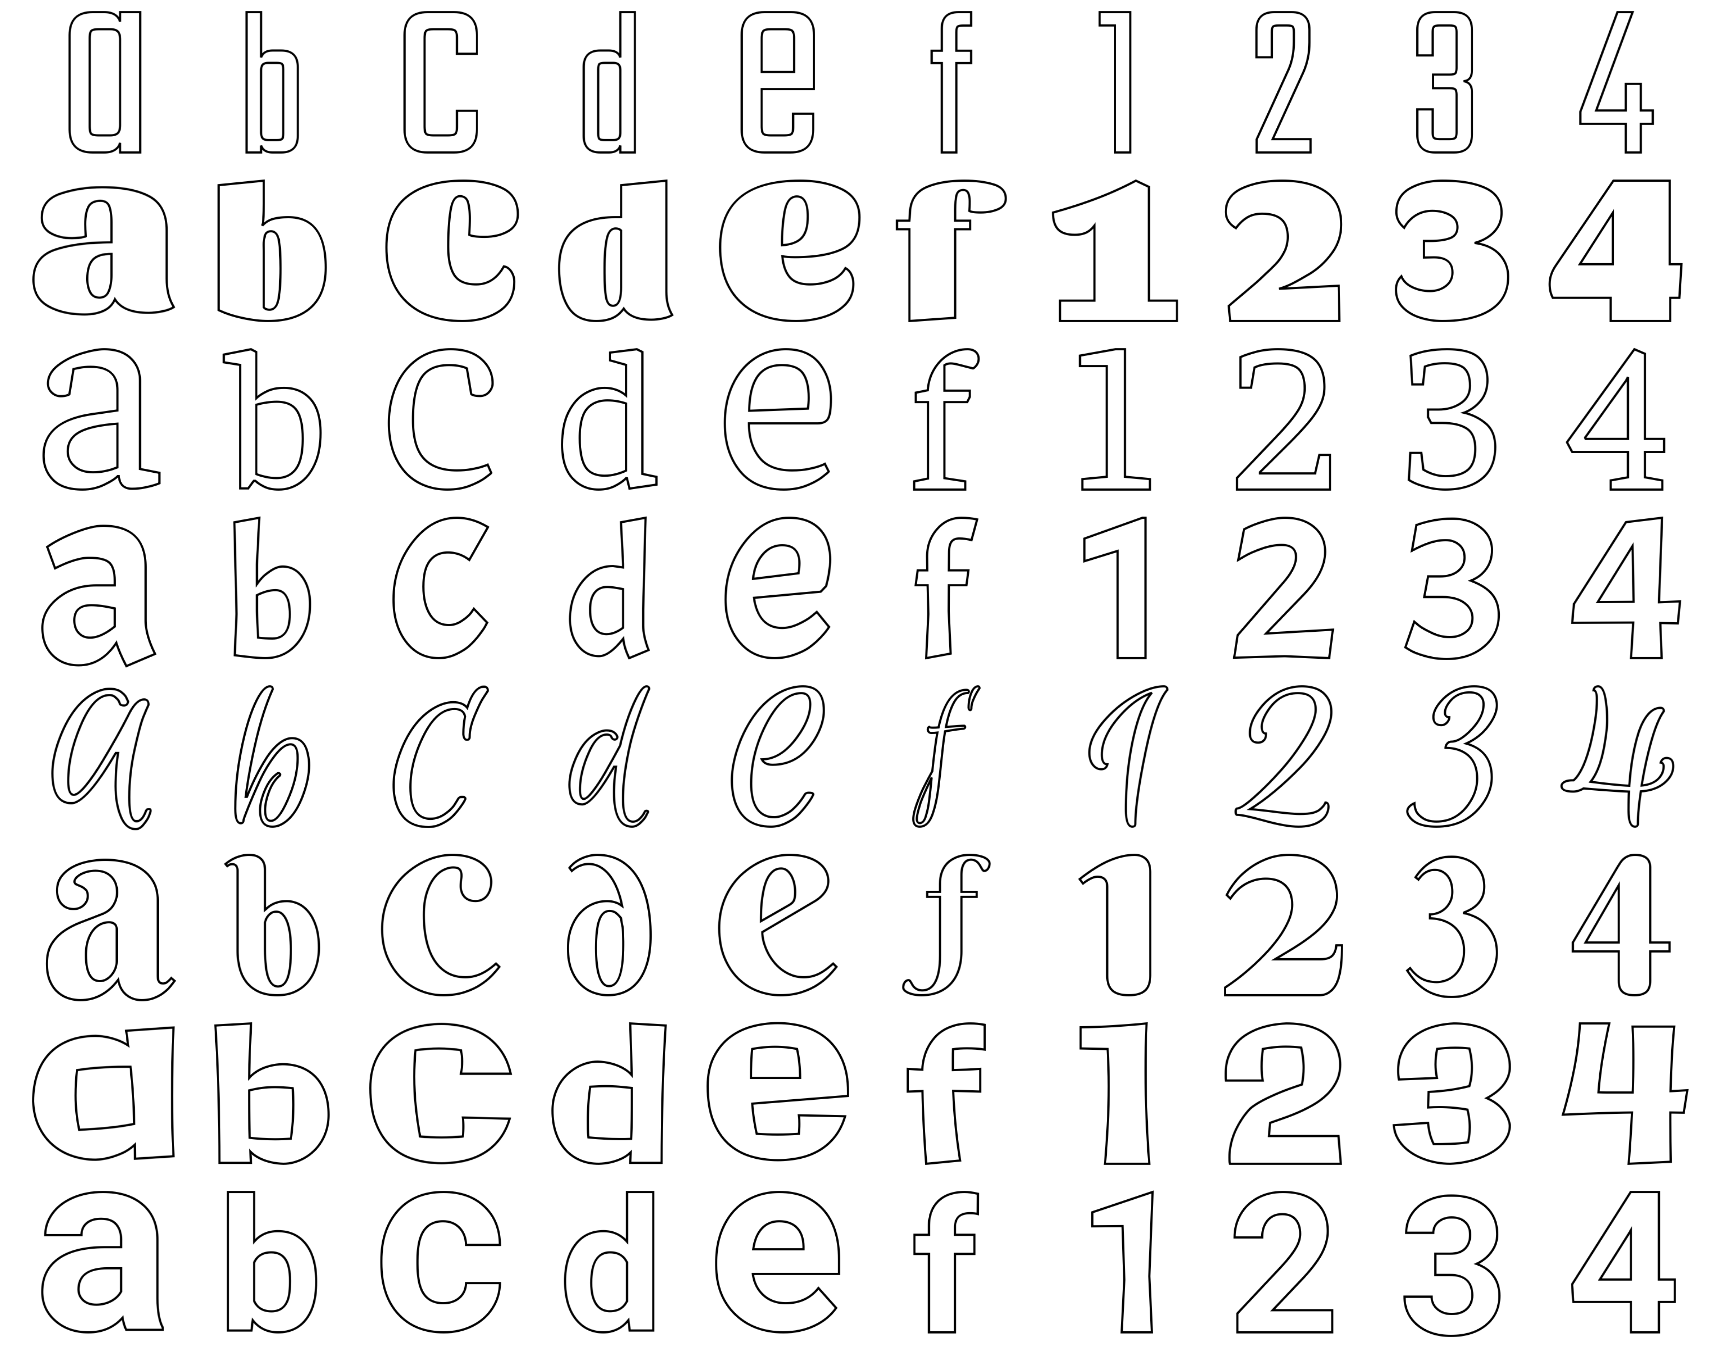
\includegraphics[width=\textwidth]{figures/input_fonts}
    \caption[A sample of the types of font faces used in our fonts dataset]{A sample of the types of font glyphs used in our dataset. Lowercase letters ``a'' through ``f'' are shown, as well as digits 1 through 4. Note the variety of styles represented: the dataset includes serif, sans serif, display, and handwriting style fonts.\label{fig:input_fonts}}
\end{figure}

\section{Generative modeling}
While discriminative modeling methods in machine learning focus on separating and identifying inputs to produce output labels learned from high-dimensional data such as images, generative algorithms create previously unseen instances of a class based on representative inputs. They are trained in an unsupervised or semi-supervised manner to model a data distribution $P$, estimating the true data distribution $P_{gt}$ from which samples are drawn. By drawing probabilistically from $P$, they can then be used to synthesize novel, unseen examples similar to input data.

Two popular neural network-based approaches include variational autoencoders (VAEs) and generative-adversarial networks (GANs)~\cite{karpathy2016generative}. Variational autoencoders, introduced in~\cite{kingma2013auto}, explicitly learn an encoder function mapping training examples from the input space $\mathcal{X}$ to a latent space $\mathcal{Z}$ as well as a decoder function mapping from $\mathcal{Z}$ to data points that are in $\mathcal{X}$ but distinct from training inputs $X$. Introduced in~\citeyear{goodfellow2014generative}~\cite{goodfellow2014generative}, GANs pit a generative model $G(z; \theta_g)$ against an adversary $D(x; \theta_g)$ that learns to discriminate samples from the ground truth dataset and the generative model's latent space. When both models are differentiable functions, backpropagation can be used to train $G$ and $D$ towards convergence in a computationally efficient manner.

More recent work in the generative direction has focused on improving the performance of these models. For example, \cite{semeniuta2017hybrid} introduces a hybrid model with two components: a standard VAE with convolutional encoder and deconvolutional decoder functions and a RNN model that takes in activations from the decoder to separate out latent text encoding from higher-level context-driven semantics. InfoGAN, introduced in \cite{chen2016infogan}, uses disentangled representations that separate salient features of inputs to learn a generative model while completely unsupervised.

\subsection{Variational autoencoders}

\section{Related work}
\subsection{Image generation}
\subsection{Font style}
